% *********************************************************************
% © 2021-2023 Jeremy Sylvestre
%
% Permission is granted to copy, distribute and/or modify this document
% under the terms of the GNU Free Documentation License, Version 1.3 or
% any later version published by the Free Software Foundation; with no
% Invariant Sections, no Front-Cover Texts, and no Back-Cover Texts. A
% copy of the license is included in the appendix entitled “GNU Free
% Documentation License” that appears in the output document of this
% PreTeXt source code. All trademarks™ are the registered® marks of
% their respective owners.
%
% *********************************************************************

\newcommand*{\xmin}{-0.5}
\newcommand*{\xmax}{4}
\newcommand*{\ymin}{-2}
\newcommand*{\ymax}{2}
\newcommand*{\func}{\x * \x}

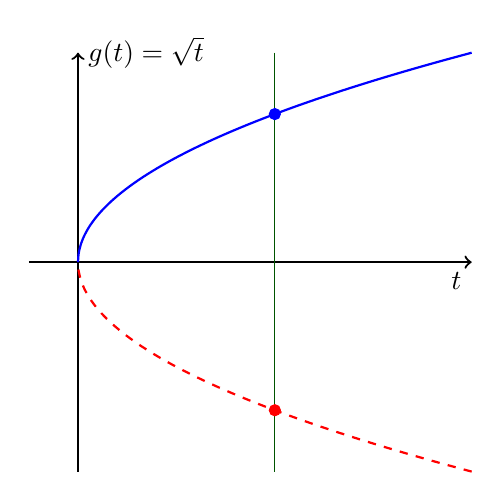
\begin{tikzpicture}
[
	closedpt/.style={circle,draw,fill,inner sep=0pt,minimum size=4pt},
	openpt/.style={circle,draw,inner sep=0pt,minimum size=4pt},
	yscale=1.33,
	xscale=1.25
]


	% axes
	\draw[->,thick] (\xmin,0) -- (\xmax,0) node[below left] {$t$};
	\draw[->,thick] (0,\ymin) -- (0,\ymax) node[right] {$g(t) = \sqrt{t}$};

	\draw[green!33!black] (2,\ymax) -- (2,\ymin);

	% graph
	\draw[red, dashed, thick, domain=\ymin:0, smooth] plot ({\func},\x);
	\draw[blue, thick, domain=0:\ymax, smooth] plot ({\func},\x);

	\node[closedpt,blue] at (2,1.414) (pt) {};
	\node[closedpt,red] at (2,-1.414) (pt) {};

\end{tikzpicture}
